\documentclass{acm_proc_article-sp}

\usepackage{algorithm}
\usepackage[noabbrev]{cleveref}
\usepackage[noend]{algpseudocode}
\usepackage{epstopdf}

\usepackage{framed}

\usepackage{xspace}
\newcommand{\ie}{\emph{i.e.}\xspace}
\newcommand{\eg}{\emph{e.g.}\xspace}
\newcommand{\vs}{\emph{v.s.}\xspace}
\newcommand{\rock}{\hbox{\textsc{rocksample}}\xspace}
\newcommand{\poc}{\hbox{\textsc{pocman}}\xspace}
\newcommand{\egreedy}{\hbox{$\varepsilon$-\textsc{greedy}}\xspace}
\newcommand{\eroulette}{\hbox{$\varepsilon$-\textsc{roulette}}\xspace}
\newcommand{\soft}{\hbox{\textsc{softmax}}\xspace}
\newcommand{\rsoft}{\hbox{\textsc{r-softmax}}\xspace}

\newcommand{\RS}[2]{%
\begin{framed}%
\filbreak
	%\noindent
\textbf{Result {#1}:~}{\emph {#2}}%
\end{framed}
}

\begin{document}

\title{Monte Carlo Tree Search Tree Policies}
\subtitle{Randomized Algorithms}
%
% You need the command \numberofauthors to handle the 'placement
% and alignment' of the authors beneath the title.
%
% For aesthetic reasons, we recommend 'three authors at a time'
% i.e. three 'name/affiliation blocks' be placed beneath the title.
%
% NOTE: You are NOT restricted in how many 'rows' of
% "name/affiliations" may appear. We just ask that you restrict
% the number of 'columns' to three.
%
% Because of the available 'opening page real-estate'
% we ask you to refrain from putting more than six authors
% (two rows with three columns) beneath the article title.
% More than six makes the first-page appear very cluttered indeed.
%
% Use the \alignauthor commands to handle the names
% and affiliations for an 'aesthetic maximum' of six authors.
% Add names, affiliations, addresses for
% the seventh etc. author(s) as the argument for the
% \additionalauthors command.
% These 'additional authors' will be output/set for you
% without further effort on your part as the last section in
% the body of your article BEFORE References or any Appendices.

\numberofauthors{2} %  in this sample file, there are a *total*
% of EIGHT authors. SIX appear on the 'first-page' (for formatting
% reasons) and the remaining two appear in the \additionalauthors section.
%
\author{
% You can go ahead and credit any number of authors here,
% e.g. one 'row of three' or two rows (consisting of one row of three
% and a second row of one, two or three).
%
% The command \alignauthor (no curly braces needed) should
% precede each author name, affiliation/snail-mail address and
% e-mail address. Additionally, tag each line of
% affiliation/address with \affaddr, and tag the
% e-mail address with \email.
%
% 1st. author
\alignauthor
Vincent Hellendoorn \\
       \affaddr{4091302}\\
       \affaddr{Msc Computer Science, TU Delft}\\
       \email{v.j.hellendoorn@student.tudelft.nl}
% 2nd. author
\alignauthor
Kaj Oudshoorn \\
       \affaddr{4009444}\\
       \affaddr{Msc Computer Science, TU Delft}\\
       \email{k.oudshoorn-2@student.tudelft.nl}
}

\maketitle

\begin{abstract}
Many intractable problems, like the Travelling Salesman Problem and scheduling problems can be sampled in polynomial time. MCTS uses this fact and applies the intuition of Monte Carlo simulations, by using repeated random samplings. Being the first to ever beat a professional Go player, MCTS is surely a promising research area. Over the years MCTS has improved even further by using so called Tree Policies instead of random sampling. These Tree Policies use a trade-off between exploration and exploitation to determine what to sample during the given timespan. We have evaluated the advantages and disadvantages of a few of these policies (UCB1, \egreedy and \soft) and have used them as building blocks for two novel Tree policies. 
\end{abstract}

%!TEX root=../report.tex
\section{Introduction}
Many problems are generally intractable due to exponentially large state-spaces. This category of problems includes both classical optimization problems, such as TSP and scheduling problems \cite{browne2012survey}, as well as two-player games such as Go, Chess and 4x4x4 Tic-Tac-Toe \cite{chaslot2010monte, sharma2008knowledge}.
Results from the ML and AI communities indicate that many of these problems, despite having exponential state-spaces, have tractable sample complexity guarantees \cite{sharma2008knowledge}. This is exemplified by the success of AI players in the game Chess (state-space $~ 2.3 \cdot 10^{49}$ positions) against human opponents, arguably culminating in the defeat of Garry Kasparov by IBM's Deep Blue AI \cite{campbell2002deep}.

Other problems have remained out of the reach of AI approaches for many decades: the two-player game Go is generally considered the last game in which humans consistently outperform computer players, having a state-space of $~2.08 \cdot 10^{170}$ positions on the default board size of 19x19 \cite{tromp2007combinatorics}. However, even on 9x9 boards, where the state-space complexity is lower than that of chess, state-of-the-art AI-approaches failed to outperform human players due to a variety of factors such as deep trees and a high branching factor \cite{browne2012survey}.

Monte Carlo Tree Search (MCTS) methods were the first to defeat human professionals in Go \cite{coulom2007efficient}, and have come to dominate the Computer Go field \cite{chaslot2010monte}. MCTS (independently proposed in the same year in \cite{coulom2007efficient, kocsis2006bandit, chaslot2006monte}), applies the intuition of Monte Carlo simulations, which work by repeated random sampling, to search trees. Monte Carlo simulations \cite{metropolis1985monte}, in turn, had previously found application in many fields as alternatives to solving mathematically complex problems \cite{liu2008monte}, \eg in evaluating complex integrals with bounded error.

The success of MCTS methods in Go, as well as its general formulation \cite{chaslot2010monte}, have sparked a variety of research into their application to different areas of both optimization problems (with varying succes, \eg \cite{rimmel2011optimization, cazenave2009monte}) and games \cite{schadd2008single, gelly2012grand}.\footnote{See http://www.ualberta.ca/$\sim$szepesva/MCTS/ for a comprehensive overview.} However, successful applications have all but consistently had to adapt the UCB1 tree selection policy, which has come to be regarded as standard, to incorporate heuristics based on the various domains, suggesting that the standard search heuristics fail to generalize well. This suggests that the standard approach fails to make optimal use of the search tree in general.

In this work, we investigate a variety of tree selection policies on small and large instances of two problems: \rock and \poc (static environment, $10^4 - 10^7$ states \vs dynamic environment, $10^{11} - 10^{18}$ states). These problems fall into the category of games with partially observable state, meaning that in general only a belief about the state of the game is known. We find that a simple technique such as \egreedy almost consistently outperforms the UCB1 search policy, particularly in the case of many simulations. Furthermore, two algorithms that behave increasingly more greedy as the number of simulations progress, in particular \soft outperform both these techniques. Finally, we propose a variation on \soft, named \rsoft, that avoids hand-tuning the \emph{temperature} parameter while performing comparable result.

\section{Monte Carlo Tree Search}

Monte Carlo Tree Search is a heuristic algorithm that is used for online planning. It is easiest explained in relation to games. Take for example a game of chess. The goal is to capture the opponents king while keeping your own king safe. However, in order to obtain that goal a number of moves have to be made by you and your opponent alternatively. Deciding which move to make, given the state of the game is key to winning the game. Moves can have direct rewards (like the capture of an opponents piece), but in general the effect of a move is only noticed a few turns after it has been made. For this reason it is hard to estimate how good a move is, without thinking a few steps ahead. Thinking ahead is, however, considerably hard, given the number of options a player has each turn. At the start of the game, a player can make 20 different moves (sixteen with pawns, four with knights), likewise his opponent also has 20 different moves, resulting in 400 possibilities in the first two moves alone. %TODO

Instead of looking through all the combinations of actions and observations, MCTS iteratively samples a selected number of actions and evaluates them through simulation. The resulting value is propagated back through the tree and updates the expected value of each action. After a number of these iterations (called simulations), the action with the highest expected reward is performed (followed by an observation) and the algorithm continues with the obtained state in order to decide the next action. Selecting the to-be-simulated action path is performed by the Tree Policy. The goal of the policy is to find a balance between exploration and exploitation. Exploration is choosing those actions that have not been sampled much so far. Exploitation is about more extensively searching in the direction of actions you already have high expectations from. 

\section{Tree Policy}

During the construction of the tree, there is one important decision to make: which path should be traversed? While deciding this at random will certainly give you some knowledge about the structure of the tree, you will not find good moves with certainty, if the amount of simulations is small in comparison with the amount of leafs. Instead it is better to use a bit of intelligence for this decision. This is provided by the Tree Policy. 

One can argue that visiting nodes that you expect to be useful will help grow confidence in your decision. By sampling different scenario's based around similar decisions, you gain more knowledge and are able to determine whether they are truly useful or not. But at the same time, there can be actions which do not seem promising at first, but can turn out to be even more rewarding than any other action. This is a trade-off between exploiting promising actions and exploring less-visited actions.

Every Tree Policy tries to cope with this trade-off. But while the ideas remain the same, the approach can be quite different. As can be seen in the following subsections, where various Tree Policies will be discussed.

\subsection{UCB1}
UCB stands for Upper Confidence Bounds. It is probably one of the most well known tree policy in MCTS, together with $\epsilon$-Greedy. For each child node $j$, the importance of visiting that child $Q(j)$ is estimated. This approximation is based on the expected value of the child and how many times this node has been visited in proportion to the other children. When for each child this has been calculated, the one with the highest importance will be chosen for the next visit. 

$Q(j)$ is calculated as follows:
\begin{equation}
Q(j) = \bar{X}_j + c\sqrt{\frac{2 \ln n}{n_j}}
\end{equation}
Where $j$ is a child node, $\bar{X}_j$ is the estimated value of $j$, $c > 0$ a constant, $n$ the amount of visits of the current node and $n_j$ the amount of visits of $j$. Notice that $Q(j)$ exists out of two parts: exploitation ($\bar{X}_j$) and exploration ($c\sqrt{\frac{2 \ln n}{n_j}}$). The constant $c$ decides how important exploration is in contrast to exploitation. 

When each value is obtained for all the child nodes, child with the maximum value will be traversed. It can be seen that $C_p$ can be adjusted to lower or increase the amount of exploration used in contrast to the exploitation of the estimated value $\bar{X}_j$.

%TODO discussion

\subsection{$\mathcal{E}$-Greedy}

Another well known method is the $\epsilon$-Greedy method. Here, the best estimated child is usually visited, but with a probability $\epsilon$ a child is selected at random, uniformly, independent of the $\bar{X}_j$.
%TODO discussion

\subsection{SoftMax}
A different approach of the $\epsilon$-Greedy method is SoftMax. However, instead of switching between exploitation an exploration with a certain probability, SoftMax starts of exploring the tree and slowly becomes more focused on promising areas. This behaviour is achieved using a variable temperature $\tau$. Together with the expected value of each child $j$, the probability $P(j)$ that $j$ is selected to be simulated is calculated as follows:  
\begin{equation}
P(j) = \frac{e^\frac{\bar{X}_j}{\tau}}{\sum_{b=1}^{n} e^\frac{\bar{X}_j}{\tau}}
\end{equation}
When $\forall i$ (child of current node) $\tau >> \bar{X_i}$, $P(j)$ will be independent of $\bar{X_j}$ and thus the decision of visiting a child will be uniformly distributed. On the other hand, when $\tau$ approaches zero, $P(j)$ will approach 1 if $\bar{X_j}$ is the highest of all children, otherwise $P(j)$ will approach 0. In this sense, SoftMax is very focused on exploration when temperature is high and becomes more greedy when temperature decreases. The tricky part of SoftMax is choosing the starting value of $\tau$ how fast $\tau$ decreases. The starting value determines how random your first decisions are and the decrease rate determines how fast you start selecting greedily. 
%TODO discussion

%!Tex root=../report.tex

\section{Experimental Setup}
We make use of the publicly available framework created by Silver \& Vennes \cite{silver2010monte}. This framework was originally developed to evaluate the performance of MCSTs on games with hidden state, using Partially Observable Monte-Carlo Planning (POMCP).

%!Tex root=../report.tex

\begin{figure*}[ht!]
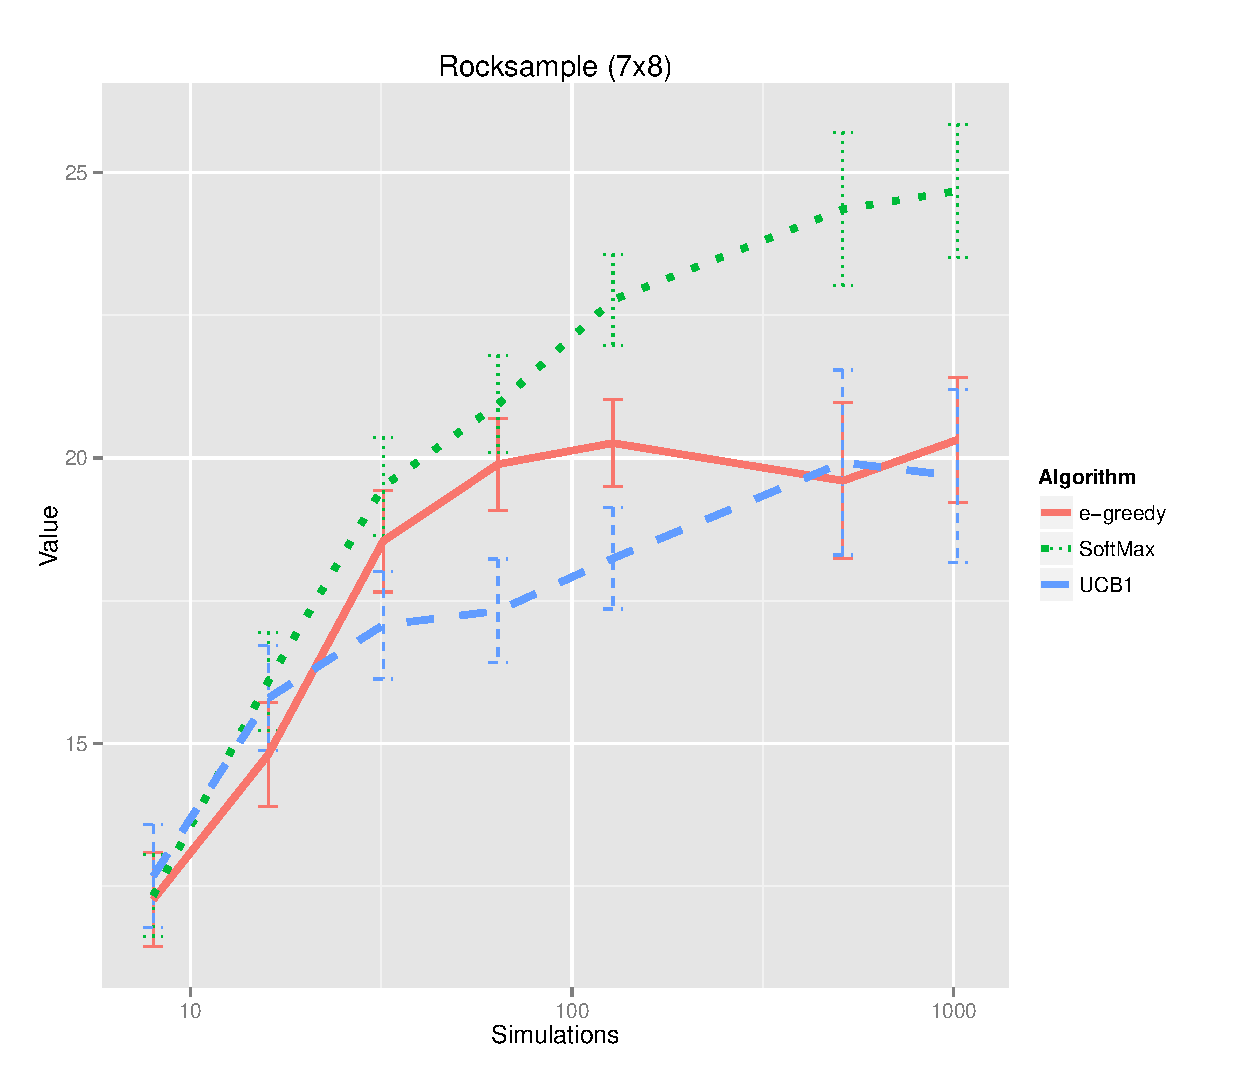
\includegraphics[width=.5\linewidth,height=.3\linewidth]{rocksample78.eps}
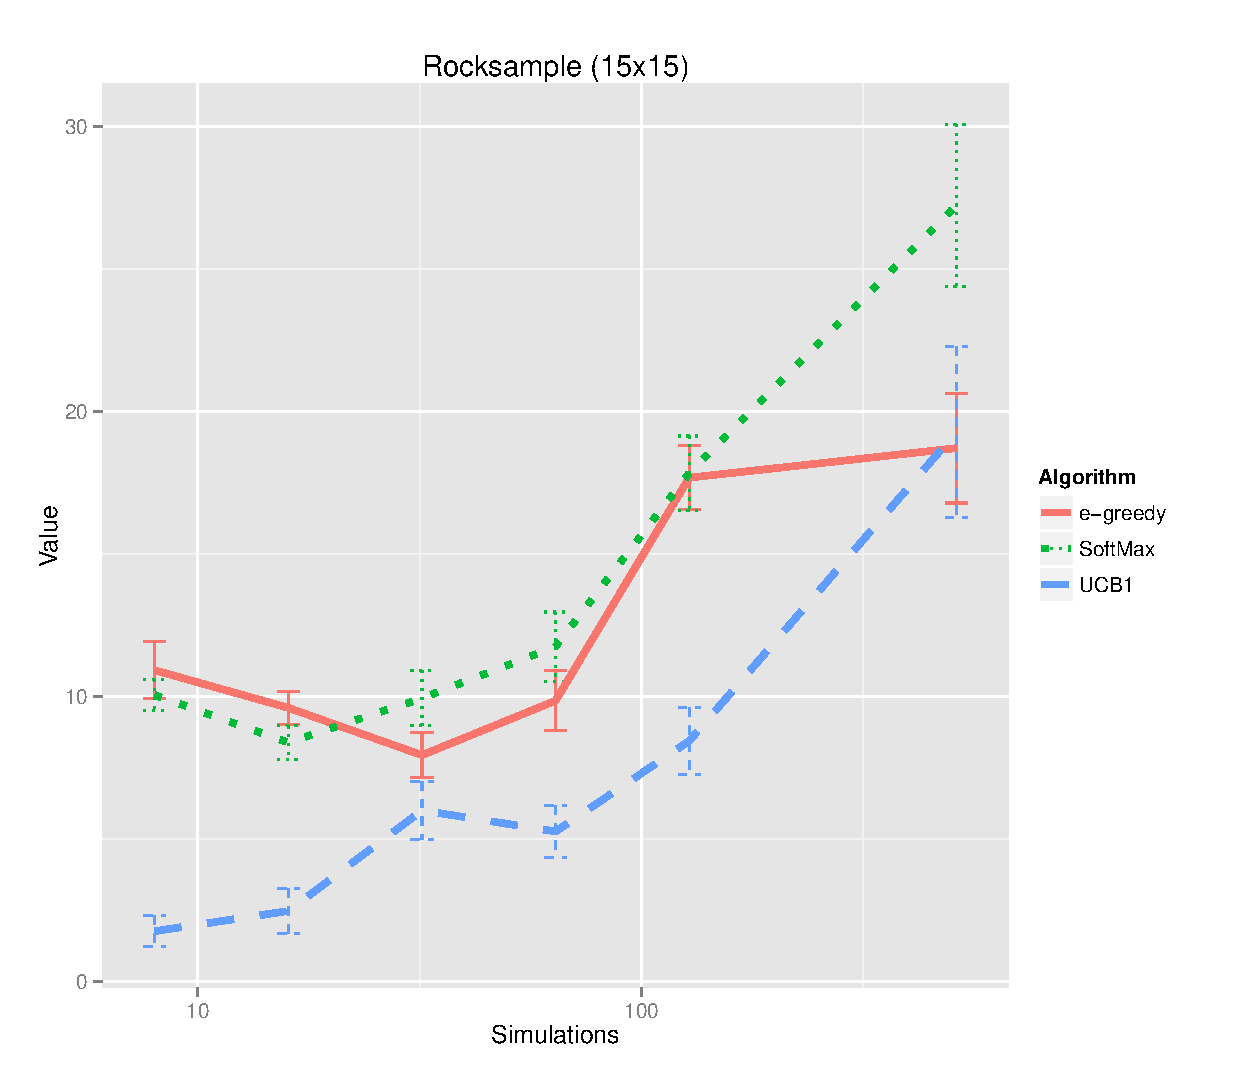
\includegraphics[width=.5\linewidth,height=.3\linewidth]{rocksample1515.eps}
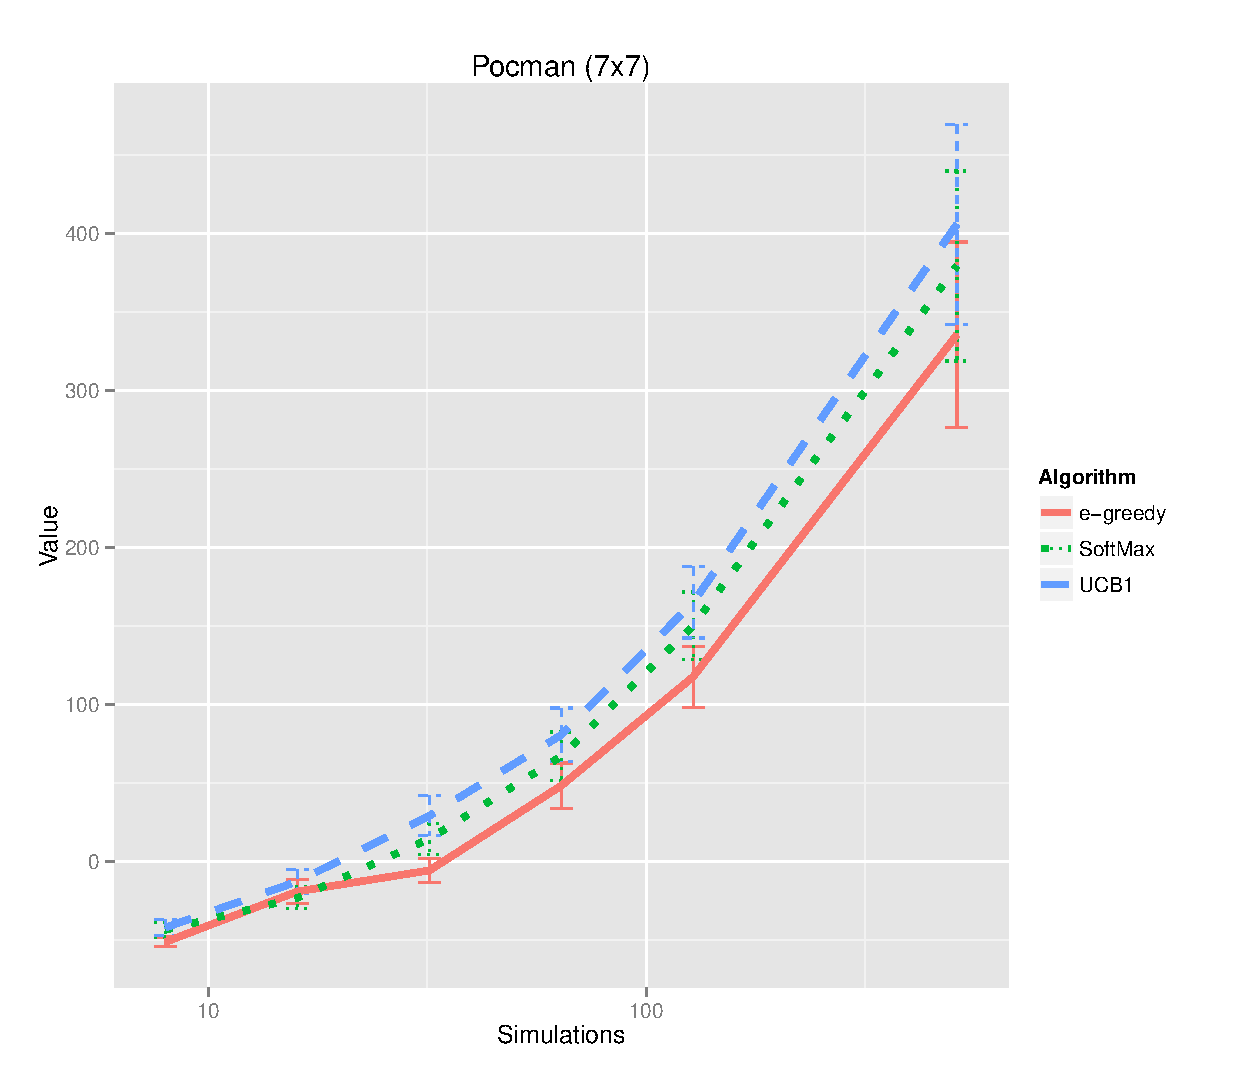
\includegraphics[width=.5\linewidth,height=.3\linewidth]{pocman77.eps}
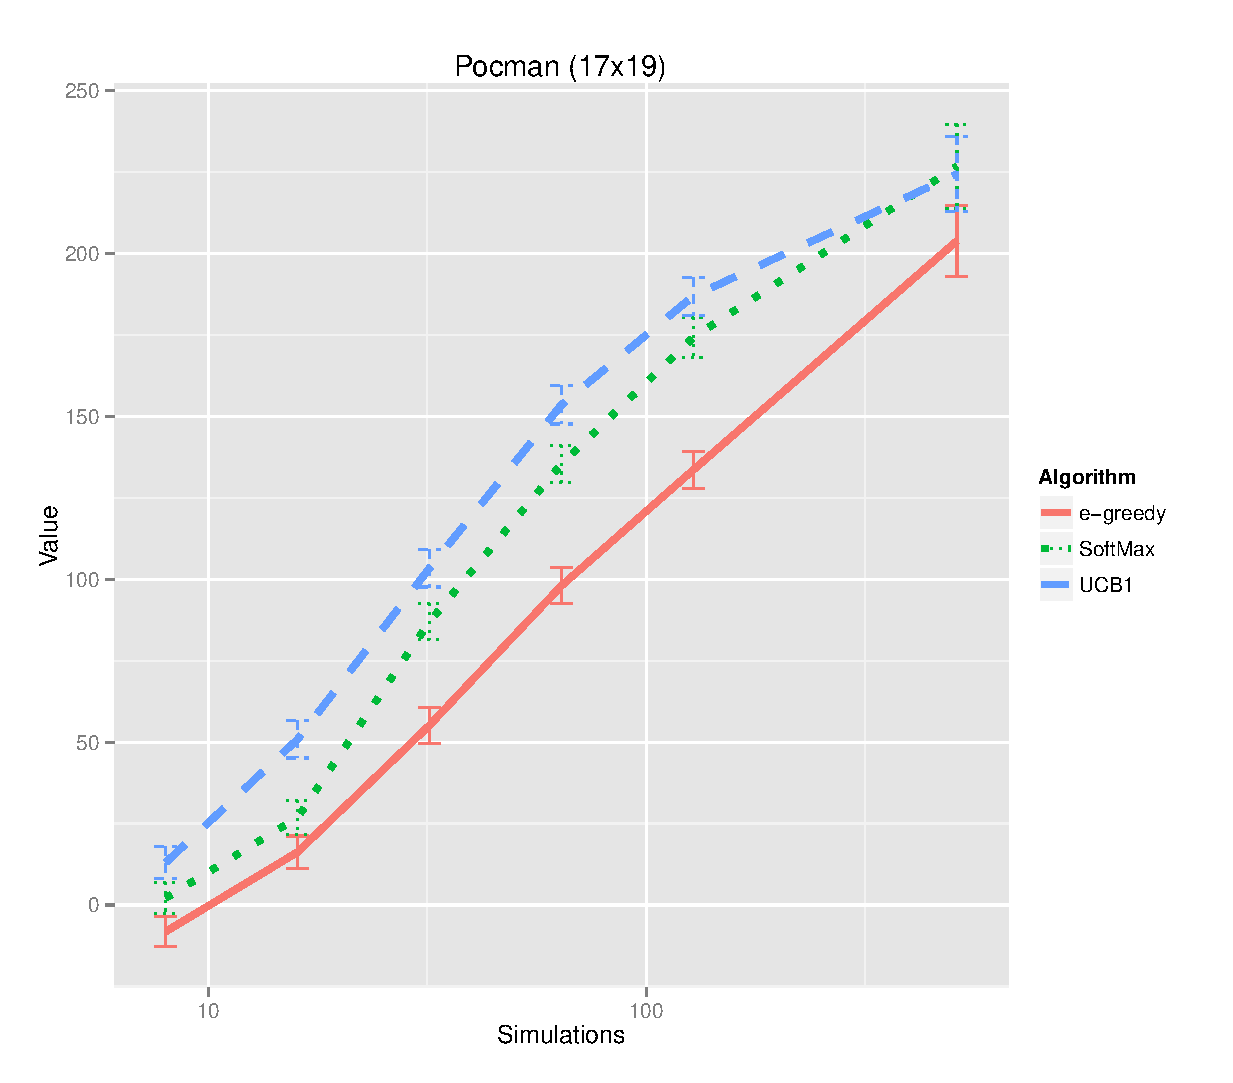
\includegraphics[width=.5\linewidth,height=.3\linewidth]{pocman1719.eps}
\caption{Comparison of UCB1, \soft and \egreedy on two \rock instances and two \poc instances. Note the log-scale on the x-axis, reflecting the increase in simulations. 95\% confidence intervals are indicated on each plot point.}
\label{fig:results1}
\end{figure*}

\section{Evaluation}
\label{sec:eval}
We conduct our analysis of the selected heuristics in three steps, investigating each of the initially studied heuristics separately. Furthermore, to better understand the reason for their relative performance, we propose and evaluate extensions for both \egreedy and \soft. Firstly, we seek to establish whether the default usage of UCB1 is justified on POMDP instances. To this end, we compare UCB1 with two commonly used general-purpose search heuristics: \soft and \egreedy on both the two instances of \rock and of \poc. The results are shown in \Cref{fig:results1}.


\subsection{Performance of UCB1}
As can be seen, performance varies substantially between \rock and \poc. In particular, all algorithms performed comparably on the \poc instances whereas larger gaps in performance were observed on the \rock instances. We identify two probable causes for this discrepancy, which both affect performance of the heuristics: firstly, the number of actions available at every step is much larger in \rock than in \poc (13 \vs 4). The impact of this difference becomes apparent when considering that each simulation recursively chooses an action up to 100 steps ahead. Whereas 256 simulation would suffice to cover all branches up to four steps ahead in \poc, it would only just suffice for two steps in \rock. The second cause lies with the presence of dynamic elements in \poc (ghosts), which may reduce the need to plan far ahead in taking actions.

Both these elements are reflected in the performance of UCB1. whereas UCB1 is nearly consistently (and often substantially) outperformed on \rock, it achieves top performance (often shared with \soft) on \poc. UCB1 will initially explore all branches but thereafter is more keen to explore branches on which it previously found good performance. This is likely inefficient when many actions are present, as is the case on \rock, as the algorithm may too eagerly give up on an action when one subsequent path leads to poor results. On \poc, however, this strategy works to its advantage, allowing it to explore a few actions in great depth. 

\RS{1}{A greedy strategy is poorly equipped when many actions can be chosen.}

\subsection{Investigating $\varepsilon$-Greedy}
Roughly the inverse of UCB1s performance holds for \egreedy. In particular, \egreedy performs worse than \soft with a greater number of simulations and worse than both other heuristics in the case of a greater state space. This suggests that a constant degree of purely random exploration is inefficient. To evaluate this hypothesis, we propose \eroulette: a variation of \egreedy in which, with probability $\varepsilon$, the action is chosen through roulette wheel sampling based on the action value of each child. We compare this variation with \soft in \Cref{fig:results2}. As can be seen, performance improves only on \rock 7x8 and severely decreases on \poc. This suggests that a greater state-space necessitates a shift to increasingly greedy investigation of a few branches towards the end of each iteration. The improved performance on \rock 7x8 furthermore suggests that a greater number of simulations is more efficiently utilized by investigating multiple branches even towards the end of the search.

\RS{2}{Greater state-spaces necessitate increasingly greedy investigation.}

\begin{figure*}[ht!]
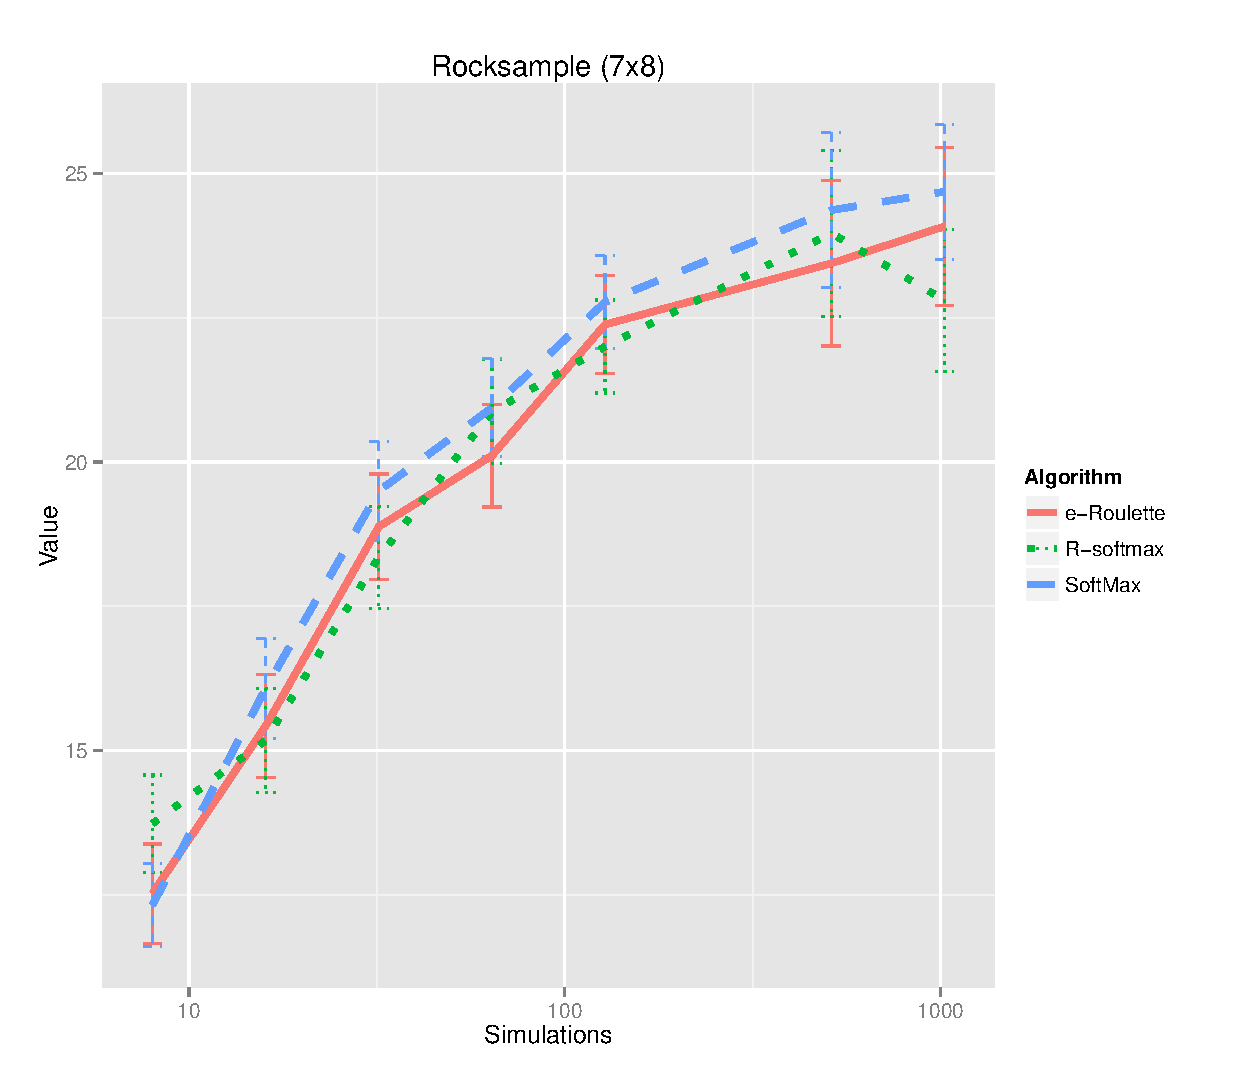
\includegraphics[width=.5\linewidth,height=.3\linewidth]{rocksample78b.eps}
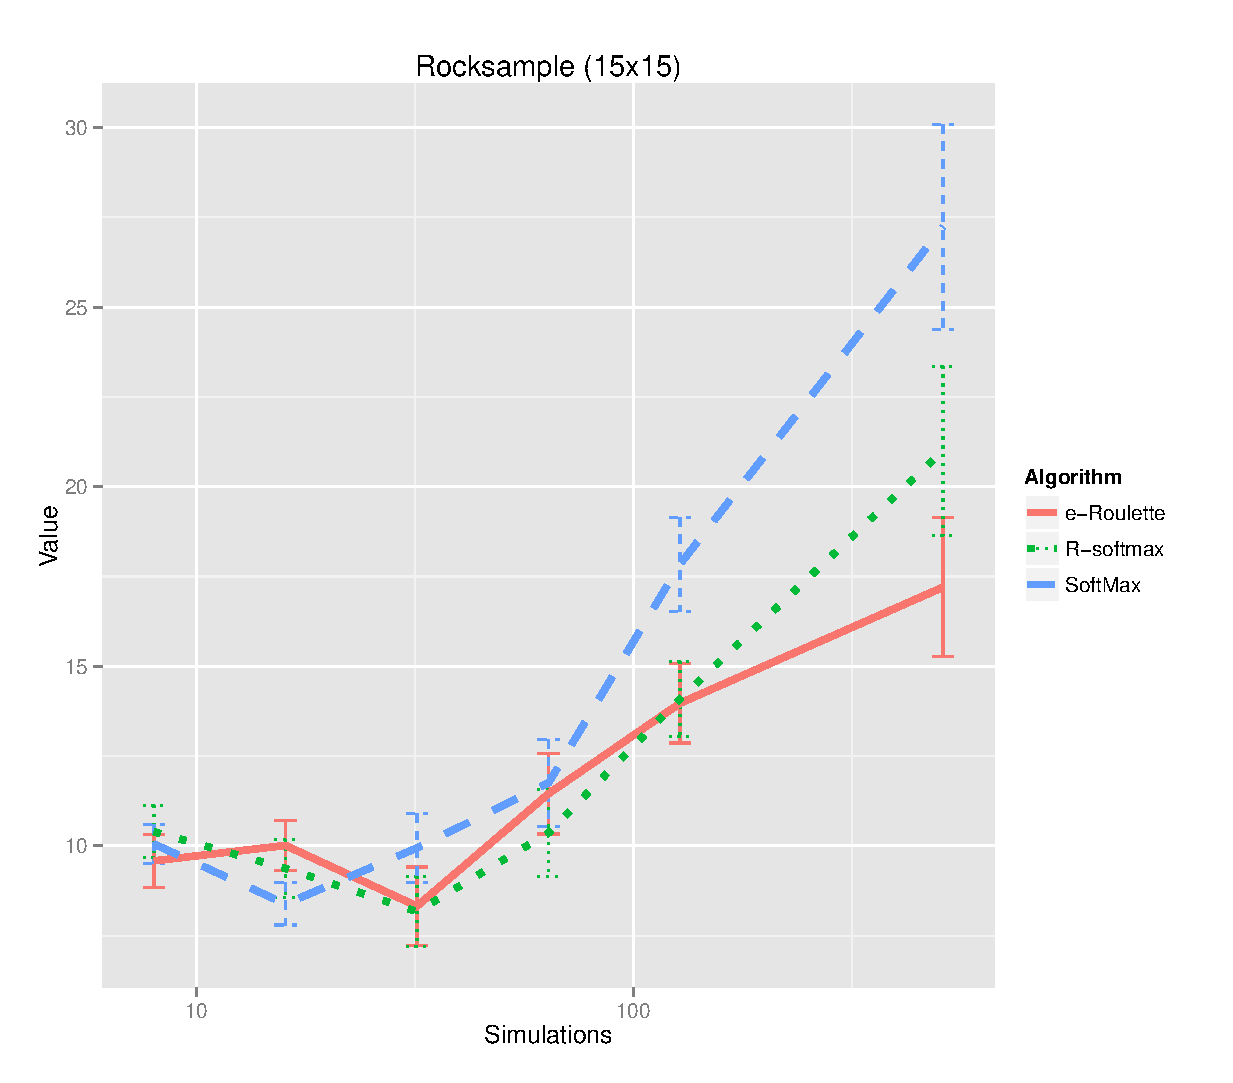
\includegraphics[width=.5\linewidth,height=.3\linewidth]{rocksample1515b.eps}
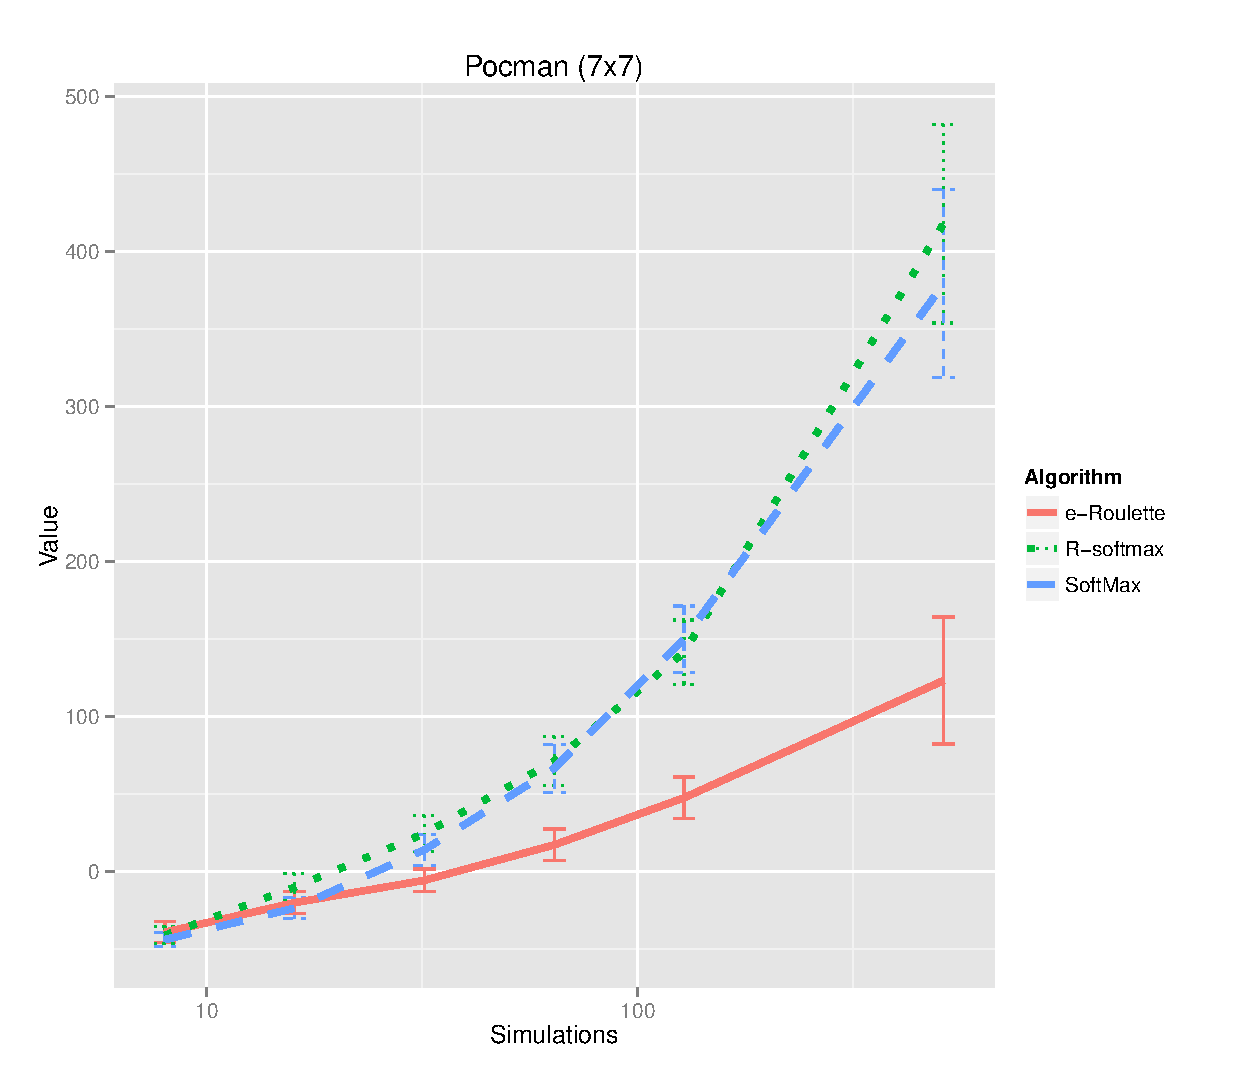
\includegraphics[width=.5\linewidth,height=.3\linewidth]{pocman77b.eps}
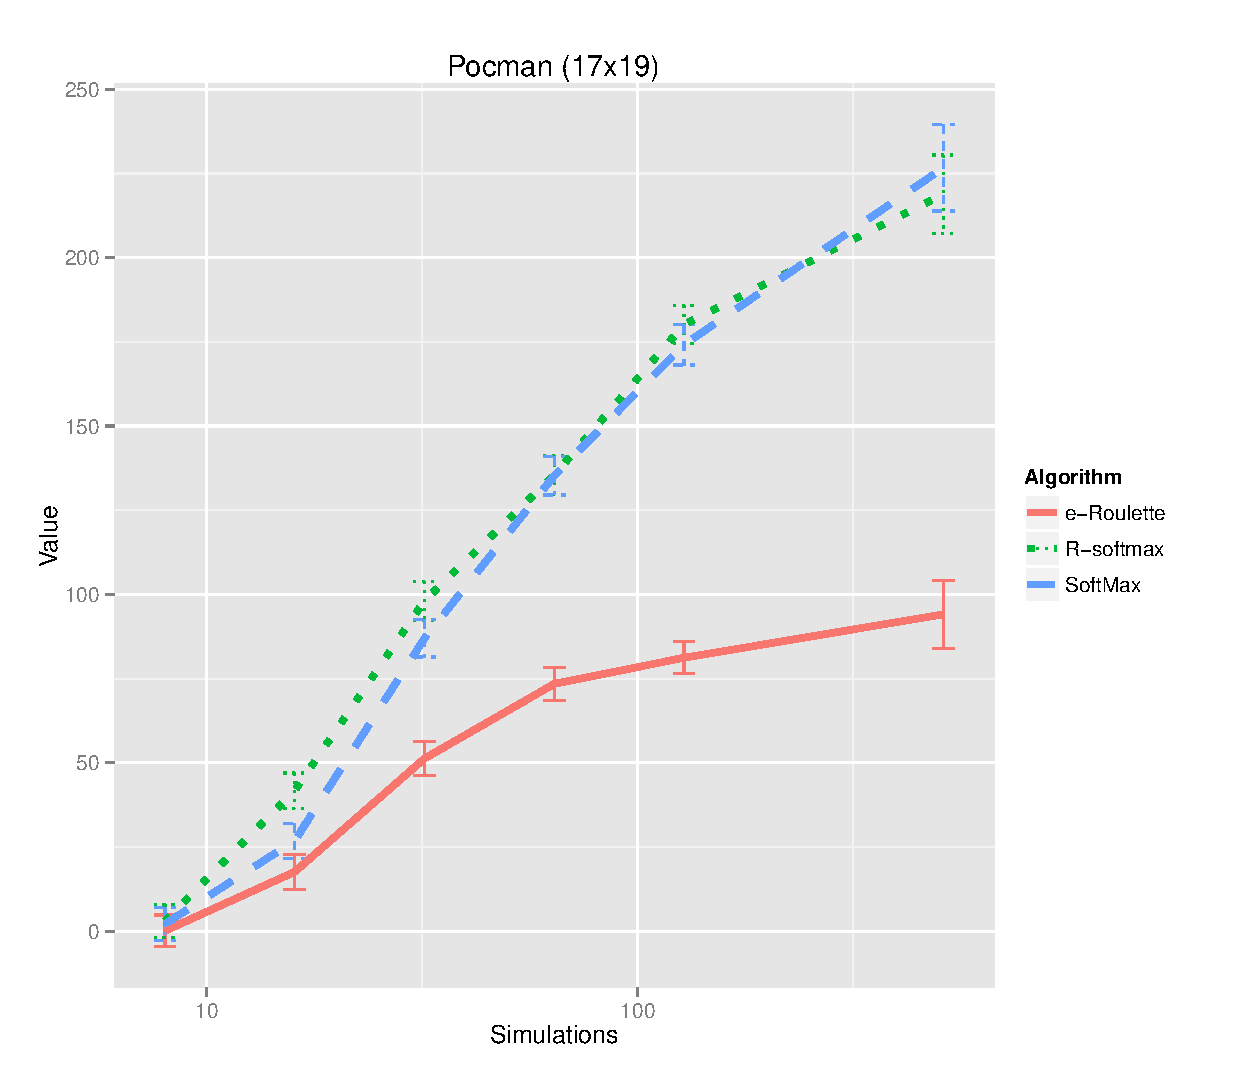
\includegraphics[width=.5\linewidth,height=.3\linewidth]{pocman1719b.eps}
\caption{Comparison of \soft to the two proposed variations: \rsoft and \eroulette, on the two \rock instances and the two \poc instances. Note the log-scale on the x-axis, reflecting the increase in simulations. 95\% confidence intervals are indicated on each plot point.}
\label{fig:results2}
\end{figure*}

\subsection{Investigating SoftMax}
In general, \soft performed best of the tested heuristics. \soft employs a temperature scheme in which the algorithm becomes progressively more greedy as the number of simulations increases. As such, it will initially visit all next actions with roughly equal likelihood, and increasingly focus its search on promising branches. Its good performs has strong implications: it suggests that the tree structure can efficiently be exploited by using the relative amount of \emph{information} present at each node (what fraction of simulations were run) to suggest the amount of \emph{randomization} with which decisions should be made.

\RS{3}{\soft yields superior performance by connecting the degree of exploration to the total number of simulations.}

As was noted in \Cref{subsec:soft}, \soft suffers from the need to manually configure the $\tau$ parameter (both start and end value), as well as the rate of decrease of the temperature. We found that this parameter was very sensitive to the actual values of actions that were present in the problem, \eg for \poc a much higher initial value was needed than in \poc as different branches of the search tree yielded potentially widely varying rewards. This creates a strong dependency on the specified rewards for each action, which in turn also adds overhead to the application of this heuristic to a new domain.

We propose a variation to \soft named \rsoft. In this algorithm, we replace each reward with its \emph{rank} in the ordered list of rewards of all children of the current node under consideration. As such, the algorithm is substantially more robust to the absolute rewards chosen. We propose to initialize $\tau$ to the number of distinct actions present, as this will start the algorithm with a high degree of random exploration. We furthermore found that the resulting algorithm is fairly robust with respect to the final value of $\tau$ and suggest setting this to $1/4$. The results are shown in \Cref{fig:results2}. As can be seen, \rsoft almost consistently performs as well as \soft (which was hand-tuned on each instance), with the exception of \rock 15x15. Future work may further investigate extensions.

\RS{4}{\rsoft sacrifices little performance in favor of broader applicability to \soft by disregarding the values of rewards used in favor of their ordering.}


\section{Threats to Validity}
This research constitutes an exploratory study of search heuristics, investigating their relative performance on a relatively small number of problems. As such, the main threats to the validity of the research described in this paper are external, reflecting the degree to which results presented here generalize to other datasets. This concerns the number of different problems investigated, the number of simulations used  and but the values of the parameters for each Tree Policy.

\subsection{Number of problems}
We have run experiments for two different types of problems belonging to the POMDP domain (\rock and \poc) with varying sizes. MCTS, however, has found application in many different domains and it is not unlikely that search trees in some other domains have fundamentally different characteristics. This is even reflected in our own experiments, where we found that \eroulette performed substantially better in \rock than in \poc. To reduce this threat, we have chosen a sample of problems and problem sizes that reflects prior work on POMDPs. Furthermore, \rsoft yielded promising results in an unrelated test following communication with E. Walraven. Further investigation of the evaluated heuristics is needed to evaluate these results on different domains. \\ \\

\subsection{Number of Simulations}
Experiments were performed using a limited number of simulations (8 to 512). These numbers have so far not been enough to show a limit on the performance for each of the Tree Policies. It is therefore unclear how the Tree Policies will behave when the number of simulations (greatly) increases. In particular, we expect some policies to end up deteriorating in performance when executed with a large number of simulations, the same behaviour that can be seen when overfitting occurs in reinforcement learning.

\subsection{Parameters for Tree Policies}
\label{subsec:params}
For the experiments, parameters needed to be chosen for the Tree policies. This concerned in particular \egreedy and \soft. For the former, we chose $\varepsilon$ (the probability of sampling an action at random) to be 0.2, after observing that it was fairly robust with respect to variations in this number. In practice, a number of ML strategies may be used to establish the optimal value for this parameter, which may benefit the performance of \egreedy. The \soft algorithm required tuning of both the start and end values of $\tau$ and the rate of decay. We found that exponential decay yielded substantially superior performance to linear decay. For the values of $\tau$, we hand-tuned the algorithm on each problem instance. Different values of $\tau$ may improve the results for different numbers of simulations as well. Given the already excellent performance of \soft, we deem it unlikely that this substantially influences the overall results.

%\section{conclusion}
In this paper, we have evaluated a number of Tree Policies that are being used by MCTS in order to solve intractable problems. This evaluation took place on the problems of \rock and \poc: two POMDP problems that cover both static and dynamic environments and represent a substantial variety in state-space sizes. By investigating three different heuristics and two newly constructed ones, we derived a number of desirable and undesirable properties for heuristics in MCTS. We furthermore found that there is room for improvement over the traditionally used UCB1 heuristic, most notably from \soft. Finally, we proposed a variation on \soft which requires less tuning while yielding comparable performance.

This exploratory study is far from exhaustive, but hopes to shed some light on the qualities of a `golden' (general-purpose) Tree Policy for MCTS problems. Future work may extend our investigation to problems that are both larger and come from different domains. Obtaining better performance may also be feasible through more investigation of the ideas behind successful Tree Policies. For instance, preliminary results indicate that taking into account the number of times that an action has already been visited, as UCB1 does, may improve the obtained results of the \soft algorithm as well. Another potentially viable option for future work is to investigate whether the algorithm should behave differently depending on how deep it currently is in the simulation tree, as deeper branches are ever less likely to be visited many times.

\bibliographystyle{abbrv}
\bibliography{sigproc}  % sigproc.bib is the name of the Bibliography in this case

\end{document}